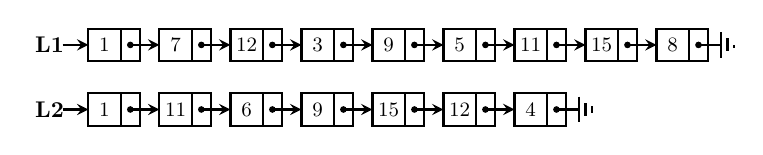
\begin{tikzpicture}[scale=0.82, transform shape, >=stealth]
    \node at (-0.6, 1) {\textbf{L1}};
    \draw[->, thick] (-0.4, 1) -- (0, 1);
    \foreach \val/\x in {1/0, 7/1.1, 12/2.2, 3/3.3, 9/4.4, 5/5.5, 11/6.6, 15/7.7, 8/8.8} {
        \draw[thick] (\x, 0.75) rectangle (\x+0.8, 1.25);
        \draw[thick] (\x+0.5, 0.75) -- (\x+0.5, 1.25);
        \node at (\x+0.25, 1) {\small \val};
        \filldraw (\x+0.65, 1) circle (1.2pt);
        \ifdim \x pt < 8.8pt
            \draw[->, thick] (\x+0.65, 1) -- (\x+1.1, 1);
        \fi
    }
    \draw[thick] (9.45, 1) -- (9.8, 1);
    \draw[thick] (9.8, 1.2) -- (9.8, 0.8);
    \draw[thick] (9.9, 1.1) -- (9.9, 0.9);
    \draw[thick] (10.0, 1.0) -- (10.0, 0.95);

    \node at (-0.6, 0) {\textbf{L2}};
    \draw[->, thick] (-0.4, 0) -- (0, 0);
    \foreach \val/\x in {1/0, 11/1.1, 6/2.2, 9/3.3, 15/4.4, 12/5.5, 4/6.6} {
        \draw[thick] (\x, -0.25) rectangle (\x+0.8, 0.25);
        \draw[thick] (\x+0.5, -0.25) -- (\x+0.5, 0.25);
        \node at (\x+0.25, 0) {\small \val};
        \filldraw (\x+0.65, 0) circle (1.2pt);
        \ifdim \x pt < 6.6pt
            \draw[->, thick] (\x+0.65, 0) -- (\x+1.1, 0);
        \fi
    }
    \draw[thick] (7.25, 0) -- (7.6, 0);
    \draw[thick] (7.6, 0.2) -- (7.6, -0.2);
    \draw[thick] (7.7, 0.1) -- (7.7, -0.1);
    \draw[thick] (7.8, 0.05) -- (7.8, -0.05);
\end{tikzpicture}
